\begin{obsolete}

\section{SOS Detector Package and Shield House }

The detector package is the key to a successful experiment. Its proper
operation should be continuously monitored during the experiments.
There are a large number of diagnostic type spectra available to aid in
this monitoring.
All the detectors are in the shield house (also referred to as detector hut).
The (concrete) shield house protects the detectors from the typical large
background environment associated with a high energy electron beam
traversing through materials (target, exit windows, possible scraping, dump).

\subsection{Shield House and Shield House Door}

The shield house interior access is covered by a two piece door. The two
halves counterweight against each other, opening vertically. The bottom
door (30 tons) is 5 tons heavier that the top door. Thus, the door will want
to open naturally if unconstrained. The door control system is used to keep
the doors closed.

The valves in the control system are set by a PLC that resides in a box
mounted beneath the stairs at the rear of the spectrometer. The front panel
of this box has two buttons for control of the door (Open \& Close),
switches for main power \& the two pumps, and several status lights. The
status lights indicate when it is necessary to clean one of the several oil
filters. The door is designed to operate electronically via a control box
mounted along the walkway near the door or from the panel beneath the
stairs. Indicator lights in the various buttons on the control box
illuminate to show the current status.

\begin{description}
\item{\bf Open} Opens the door, electronically activating the hydraulics.
Pressing this switch will illuminate both buttons on the operator panel and
on the
control box. The door will require about 60 seconds to open.
\item{\bf Close} Closes the door, electronically activating the hydraulics.
Pressing this switch will illuminate both buttons on the operator panel and on
the control box. The door will require 60 seconds to close.
\item{\bf Emergency Open} Used only if the hydraulic system fails but electrical
power is available. (i.e. hydraulic pump failure) This button operates
valves so that hydraulic fluid slowly exits the door cylinders and allows the
doors to open. Opening the door this way may require several minutes.
This switch is not spring loaded and will have to be manually reset before
other operations can continue.
\item{\bf Emergency Stop} Stops the movement of the door regardless of
direction.
This switch is not spring loaded and will have to be manually reset before
other operations can continue. Resetting the switch does not resume door
motion. Another button must be pressed to start movement again.
\item{\bf Standby} Once the door is stopped, standby may be used to keep
the door
within 0.5" of its' present position. This switch is disabled during door
movement. If the doors creep through fluid leaking by the seals in the
cylinders while the system is in standby mode the pumps will activate and the
slippage will be corrected. The cleaner the system and newer the cylinder
seals the less this slippage will occur.
\end{description}

The circuit for the door controls is located in boxes C-UPH3 (pumps, circuits
20,22,24) and C-UPL3 (120V, circuit 35).

The control panel controls:

\begin{description}
\item{\bf Open} Same as above.
\item{\bf Close} Same as above.
\item{\bf Large Grey power switch} Switches on power to electronics and pumps.
\item{\bf Pump 1, Pump 2} Each pump may be enabled individually. These two
switched do not start the hydraulic pumps.
\item{\bf On} Starts the enabled hydraulic pumps.
\item{\bf Off} Stops the enabled hydraulic pumps.
\end{description}

\subsection{Opening/Closing SOS Shield House Doors}

To open SOS shield house doors, first confirm appropriate breakers in
breaker panels on right side of carriage are "on". Open doors on power
panel at right rear of carriage, then close right hand door, making sure
that switch handle on outside of door engages switch shaft. Leave left door
open.
Operate switch handle to turn on 480 volt power. Watch message panel on
orange plc box near left end of top row of modules. Message panel should be
blank. If any message appears, {\bf STOP} and call/page Hickson or
Vulcan.  If panel is
blank, proceed. On exterior of right hand door, select either pump \#1 or
pump \#2, then press green "on" button below pump selector switches. Note
sound of pump. Go up S.O.S. stairs to walkway in front of doors. Insert
enable key in control box, and turn to "on" position. Press and hold "open"
button. Button must be depressed for - 5 minutes, 40 seconds to open doors
completely. While opening doors, watch door hydraulic cylinders; cylinder
movement should be synchronized. lf differential movement is observed,
release "open" button, hit "emergency stop'' button and call/page as 
above.  Doors will stop automatically at full open position.
If doors will be open for more than a few minutes, return to floor level
power panel and turn pump off with red "off' button below pump selector
switches, then turn off 480 volt power with switch on exterior of right
hand door. If pump is left on, close doors by pressing and holding "close"
button for - 5 minutes, 40 seconds. Doors will stop automatically when
fully closed.  When doors are closed, turn enable key to "off' and remove
key from control box. Return to 480 volt panel, turn off pump, and turn off
480 volt power. If 480 volt power was turned off while doors remained open
for an extended period, 480 volt power must be turned on to close the doors
as described above. Always observe message panel on plc after turning on
480 volt power. Never proceed If any message is displayed.

NEVER LEAVE 480 VOLT POWER ON DURING BEAM PERMIT.

NEVER USE "STANDBY" MODE.



\paragraph{Safety Items}

With the loss of electrical power all valves close automatically. This will
stop all movement of the door. The fluid in the cylinders may slowly leak
past the seals causing the door to open.

A section of handrail will be (is) attached to the downstream end of the
flip-down section of walkway. This handrail will block access to the doors
until the doors open completely and the flip-down walkway can be rotated
over the lower door.

The toe kick around the roof of the shield house will be (has been)
extended to 8", and sealed to contain fluids in the event of a catastrophic
hydraulic leak. The enclosure should capture 330 gallons of fluid adequate
to contain a complete system rupture.  The most common mode of fluid
loss is a slow drip at a joint. Rupture of a hose, while very unlikely, can
result in loss of fluid in that hose. Pressure indicators in the system
will stop
the system if loss of pressure is detected. See the hydraulic diagram for
the location of the pressure indicators (Figure~\ref{fig:SOSdoorHydSym}: explanation of symbols,
and Figure~\ref{fig:SOSdoorHydDiag}: the hydraulic diagram).

Filter replacement is required when the maintenance light on the control
panel is illuminated. The filter elements are placed between two isolation
valves. The two valves must be closed, and the pressure released before
the filter cover is removed. The filter cover is a screw on/off type. The
elements are not disposable and are designed to be cleaned and replaced.

\subparagraph{Filter Removal}

\begin{enumerate}
\item{Turn off the power to the control system.}
\item{Close the valves on either side of the filter to be replaced.}
\item{Release any built up pressure in the filter and neighboring pipe by
opening the pressure relief needle valve at the filter. Be careful of any fluid
released through the valve. {\sl The released fluid should be captured and
disposed of properly.}}
\item{Unscrew the filter cover.}
\item{Service the filter.}
\item{Replace the filter and cover.}
\item{Close the pressure relief needle valve.}
\item{Open the valves on either side of the filter.}
\end{enumerate}

\subparagraph{Valve Failure}

The solenoid valves have lifetimes of many thousands of cycles.
In a valve fails, the two pressure indicators will start to differ, soon
resulting in a too large difference between the two decoders (one for each
side of the door), causing the motion mechanism to stop.

\subparagraph{Cylinder Failure}

In the unlikely event of a cylinder failure, the door will slip slightly to one
side in the track and any motion will stop.

\paragraph{Manual Door Operation}

In the event that electrical power is lost (and thus hydraulic control) the
door can be opened manually. There are five manual popet valves, that are
to be opened in a certain sequence, that will allow hydraulic fluid to slowly
drain from the cylinders thus opening the doors.

\begin{enumerate}
\item{Open the popet valve at the top of each door cylinder (valves SV-C-9
\& SV-C-10) by
pressing the switch on the valve. The valve is located on the downstream
side at the top of each cylinder.}
\item{Open the popet valve at the bottom of each cylinder (valves SV-C-11
\& SV-C-12) in
the same way. The valve is located on the upstream side at the bottom of
each cylinder.}
\item{Finally open the valve (valve SV-C-13) located on the rear wall of the
spectrometer, above the electronics hut.}
\end{enumerate}

The fluid drains from the cylinders slowly. Opening the door this way may
take more than several minutes. The five solenoid valves will need to be
reset before electronic operation can resume.

\subparagraph{Pump Failure}

The hydraulic pump has two motors that are independently switched.
Either will provide adequate power to operate the SOS door hydraulics. It
is recommended that both pumps be used or alternated so that both are kept
lubricated.

The motion of the door is monitored by the control system. Linear
displacement encoders on each cylinder provide analog signals to the controls.
The two cylinders must move at the same rate or the control system will
stop the door progress. The doors will stop if the difference between the
cylinders becomes more than 0.020". The control system will attempt to
level the door and continue, massive skewing of the door will cause the
door to wedge in the track. If the door wedges in the track crane support
may be necessary to correct the problem.


\begin{figure}
%\htmlimage{scale=2.0,thumbnail=0.5,flip=r270}
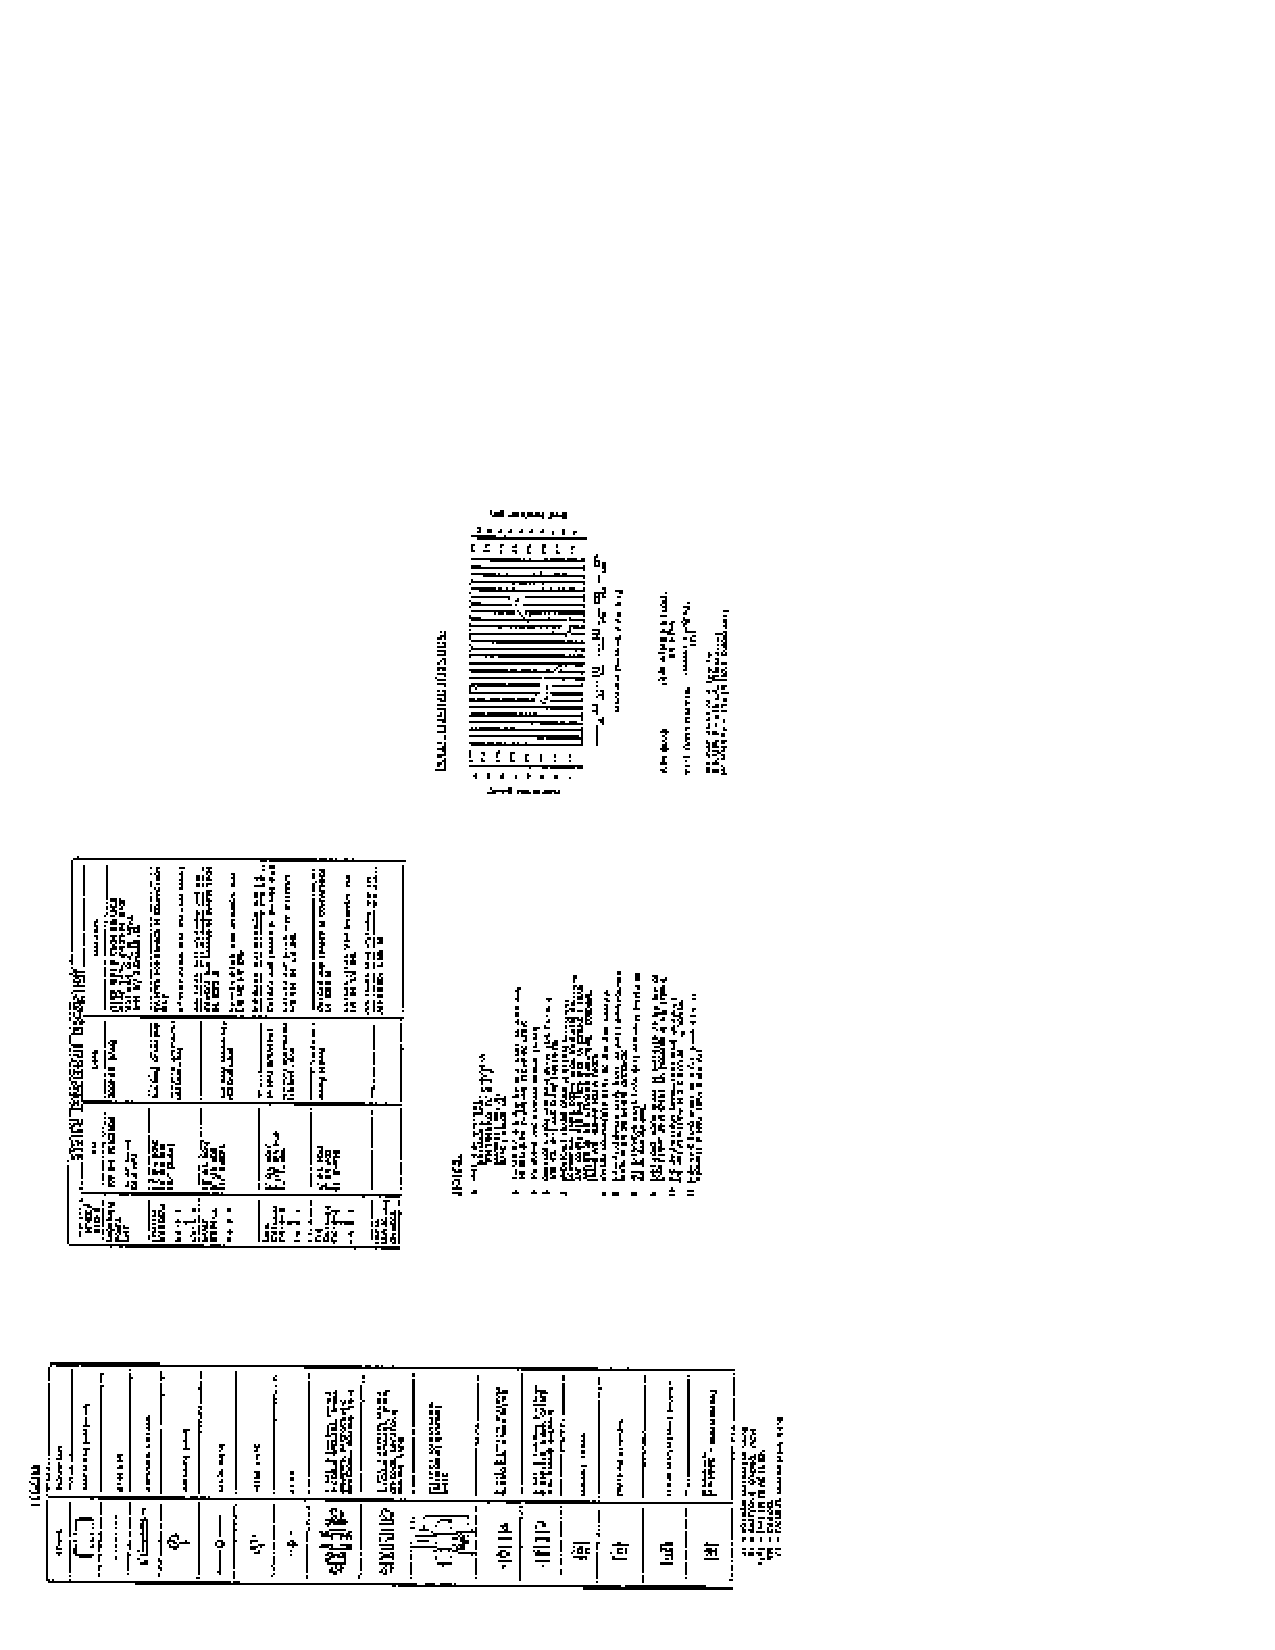
\includegraphics[height=7.2in,width=6.25in]{SOSdoorHydSym.pdf}
\caption{Explanation of Symbols used in Door/Jack Hydraulic 
Diagram. \label{fig:SOSdoorHydSym}}
\end{figure}
\clearpage

\begin{figure}
%\htmlimage{scale=1.0,thumbnail=0.5,flip=r270}
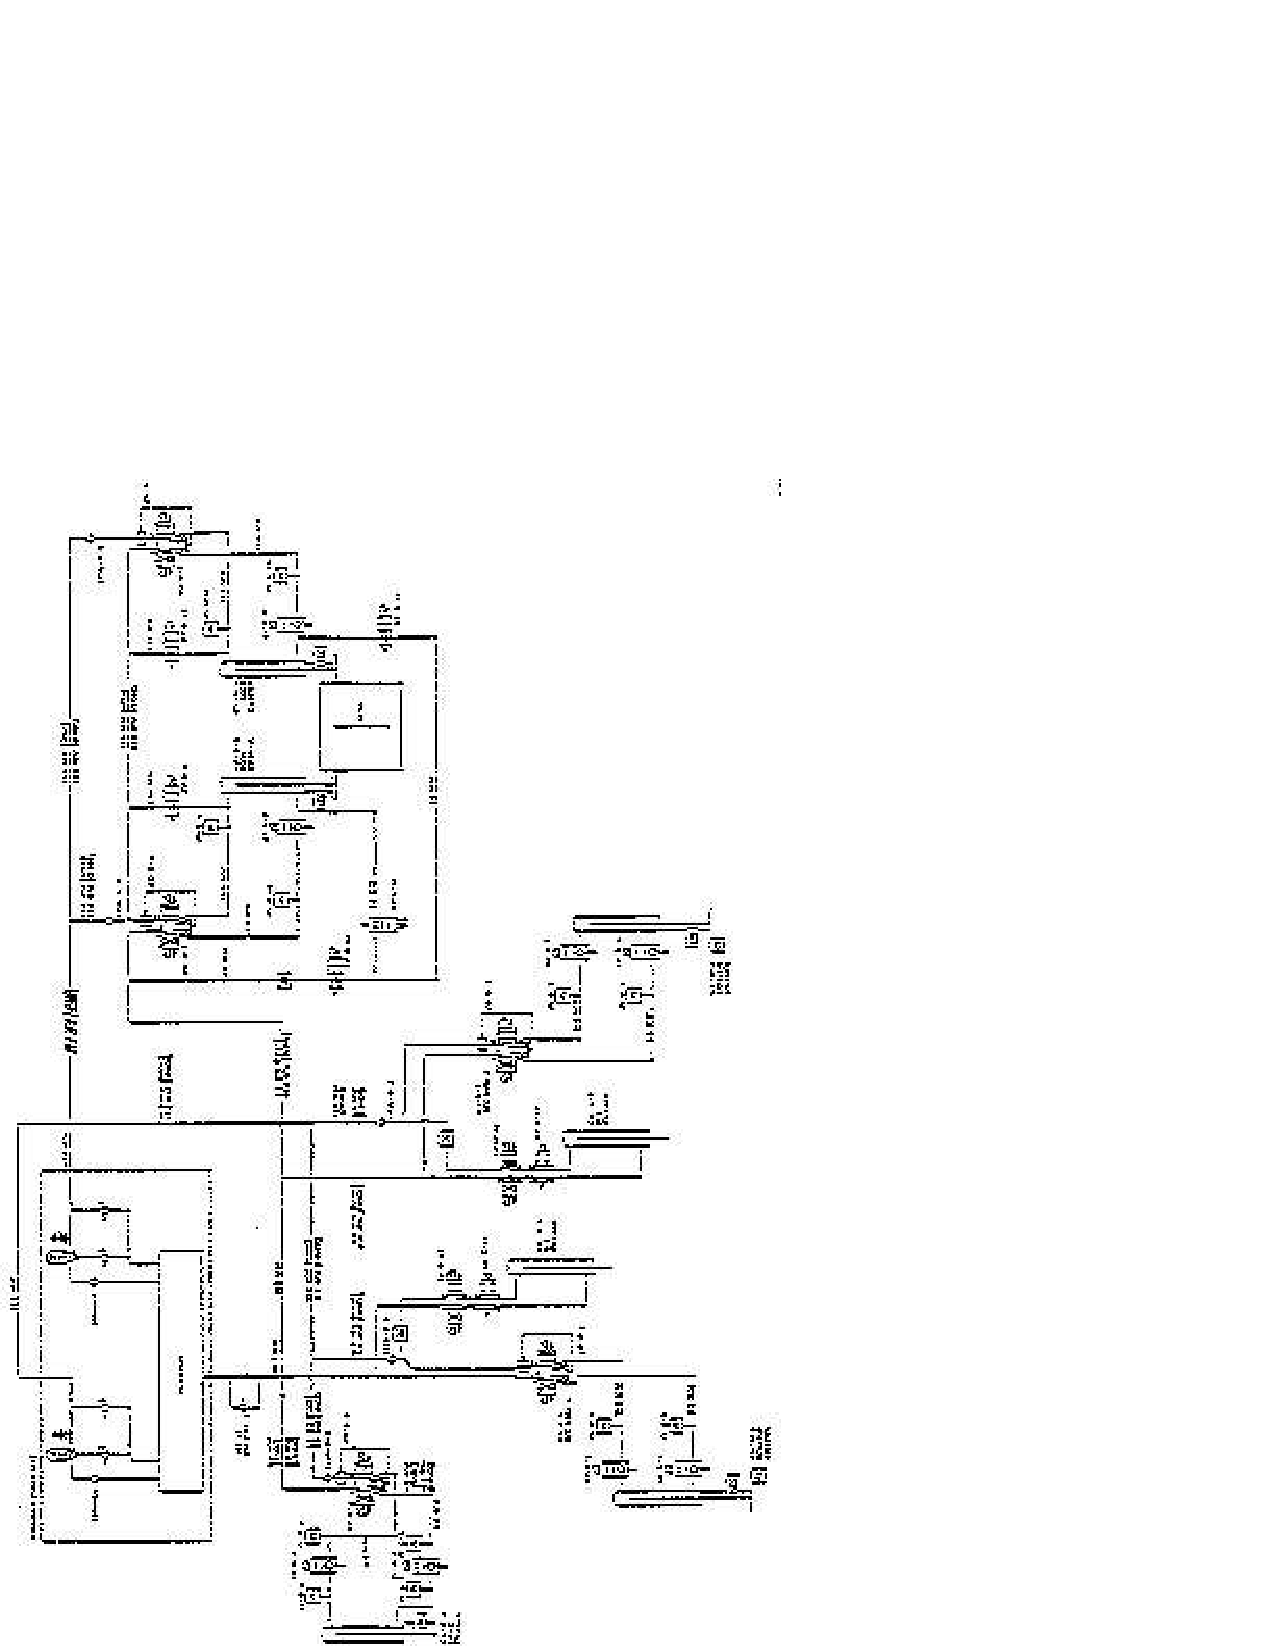
\includegraphics[angle=270,width=6.25in,totalheight=7in]{SOSdoorHydDiag.pdf}
\caption{The SOS Door/Jack Hydraulic Diagram. \label{fig:SOSdoorHydDiag}}
\end{figure}
\clearpage


\subsection{High Voltage Supplies }

All the detector elements require the use of High Voltage. The
high voltage supplies for the detectors are located in the 
electronics room of the counting house.
During experiments the control of the high voltage supplies is done via
computer and a display is available on one of the xterms around
the console in the Hall~C counting house. The control is via
EPICS and includes a graphical display so that the status of each
HV channel can be seen at a glance. Operating instructions are
in section~\ref{par:hv_ops}. {\em Typical} high voltages for
SOS detector elements are shown in Table~\ref{tab:sos_hv}.

\begin{table}[!hbt]\centering
   \caption{SOS Detector {\em Typical} High Voltages\label{tab:sos_hv}}
   \begin{tabular}{lrr}
      Detector & Voltage (V) & Current (mA)\\
      \hline
      Lucite         & 3000  & 1.0 \\
      Aerogel        & 2590  & 1.2 \\
      Gas Cherenkov   & 2875  & 2.2 \\
      Scintillators  & 2500  & 2.1 \\
      Shower Counter & 1350  & 2.1 \\
      \hline
   \end{tabular}
\end{table}

As a general rule no work should be done on detectors which are under
High Voltage and
High Voltage cables should never be removed or installed while the supply is on.
General information about the use of the {\em CAEN} power supplies can be
found earlier in this chapter.


\subsection{Drift Chambers}

\paragraph{Overview}

The drift chambers provide accurate measurements of the particles
position and angles in the detector hut. This information can be combined
with a knowledge of the spectrometer optics to infer the trajectory of the
particles at the target.

The multi wire Drift Chamber module consists of six planes of gold-plated
tungsten wires of two thicknesses: 30 $\mu$ wires held at ground
potential, and 60 $\mu$ wires held at high (negative) potential
($\left|V\right|\le3$kV).  Alternating with the wire planes are six
foil planes of 1/2 mil mylar, coated on both sides with 1200 angstroms
of copper.

The high voltage (HV) system provides the correct potentials on the
cathodes (field wires and foil planes) of the DC modules.  The HV
system is supplied by CAEN high voltage, low current power supplies.
The supplies are located in the electronics room of the counting
house. They are connected to the detectors through a high voltage patch
system from the counting house to the shield house
and coaxial cables with standard SHV connectors from the patch system
to the drift chamber modules.
The highest operating voltage in use presently is -2100 V.

Each anode wire has its own electronic readout through
Nanometrics preamplifier/discriminator
cards or LeCroy Corporation LRS 2735DC cards which are interchangeable
with the Nanometrics cards.  Each of these Drift Chamber cards has 16 inputs
which accept negative signals from the anodes (sense wires), amplify
and then digitize the signals according to whether a user-specified
threshold level is crossed.  This threshold level is set using a low
voltage (0 to 10 volts) dc power supply.  A
multi wire cable connects this threshold power supply to the Drift Chamber cards.
Each of the Nanometrics or LRS cards requires approximately five volts
(bipolar) and approximately 1/2 A.  This power is supplied by Acopian
supplies.  Each discriminator
output is connected by 34-pin (17 pair) twisted-pair cable to an LRS
1887 96 channel pipeline FASTBUS TDC.

The chambers use a 50:50 mixture (by weight) of
argon and ethane gas.  The gas is mixed in a specially-built Gas
Handling System which passes the mixed gas through an alcohol (ethanol) bubbler before
passing it to the chamber.
The gas flow is approximately 100 SCCM.

\paragraph{Personnel and Troubleshooting}

There are not many problems associated with the chamber that are
easily diagnosed from within the counting house.  The main problems
that can be addressed are empty gas bottles (replace them) and tripped
voltages (reset them). All permanent members
of the Hall~C physics and engineering staff may change gas bottles.
If the gas lines become clogged, the high
voltage should be turned off; however, there is currently no way to
monitor the gas flow without going into the detector hut.
Consequently, the gas flow should be checked during routine entries.
If the gas is not flowing, one of the lines is probably clogged.
Contact one of the SOS chamber experts (listed in the Responsible Personnel
section of the 
\htmladdnormallinkfoot{ESAD}{http://www.jlab.org/Hall-C/document})
 for further instructions.

\paragraph{Gas Flow Operation Procedures}

The gas used in the SOS drift chambers is a 50-50 mixture (by weight)
of argon and ethane.  Each chamber has a volume of approximately 13
liters, and is operated at slightly above atmospheric pressure.  When
the gas is flowing through the chambers, the windows of the chambers
will bow out slightly.

The gas bottles sit immediately outside the gas shed, which is outside
the counting house.  The pressure in the argon bottle should be
monitored daily; when it reads below 500 psi, the bottle should be
changed.  Since the ethane bottle contains compressed (liquid) ethane,
the pressure reading is not directly useful.  However, the bottle sits
on a scale.  An empty bottle weighs approximately 120--140 lbs.  When
the weight of the bottle approaches this value, the ethane bottle is
nearly empty and should be changed.  Note that since ethane is a
flammable gas, the regulator on the bottle has reversed threads.  Full
bottles of both argon and ethane should be in the same area as the
bottles in use.  

Normally, Hall C technical staff routinely checks gas bottles and
replace empties.  Experimenters are responsible for verifying and
recording gas status.  

The gas handling system (GHS) is located inside the gas shed.  It
mixes the argon and ethane in the desired proportion, and bubbles the
mixture through alcohol at 0$^\circ$C before the gas goes down into
the hall.  There are four ``channels'' (gas lines) in the system;
channels 1 and 2 are for SOS, and 3 and 4 are for HMS.  The channel is
selected with the left/right arrow keys.  The selected channel may be
turned on or off with the up/down arrow keys, which perform the same
function.  {\em Note that the on/off buttons do not control whether
the gas is on or off}.  Changing the gas flow is accomplished by
moving the cursor to the setpoint value of interest, and typing in the
desired value on the numeric keypad.  Typical values used for SOS are
200 SCCM.

To turn on the gas to the SOS drift chambers, use the following
procedure:

\begin{itemize}
\item{Ensure that the gas lines are connected to the chambers.}
\item{Ensure that the gas bottles are full.}
\item{Turn the gas flow on for channels one and two.}
\item{Set the gas flow on both channels to 200 SCCM.}
\item{After a few minutes, verify the flow rates on the flow meters at
      the chambers of 0.1--0.2 liters/minute.  If this is not the
      case, one of the gas lines is probably clogged.  See the {\em
      Troubleshooting} section for more details.}
\end{itemize}


\paragraph{High Voltage Operation Procedures}

The high voltage for the SOS drift chambers is supplied by a CAEN
high voltage power supply in the electronics room of the counting
house.  The voltage is controlled using the
high voltage GUI running on an  X-terminal in the counting house.
Instructions for using this system are in section \ref{par:hv_ops}.
The operating
voltage for the chambers is 1975V (foil) and 1975V (potential
wires).

At the start of an experiment, first ensure that the gas system is
turned on and gas is flowing through the chambers using the procedures
in the last chapter.  If the system has been off for an extended
period, gas should be flowing for at least 4 hours before high
voltage is turned on.

Control of the CAEN high voltage supplies is performed through
a GUI. See section \ref{par:hv_ops} for operating instructions.

\paragraph{Low Voltage Operation Procedures}

The low voltage for the SOS drift chambers is controlled by two
Acopian power supplies.  One provides +5V, and the other provides -5V.
The two supplies are located on SOS itself, in the level with the
electronics.  The only control on these supplies is an on/off
switch.  For normal operation, both switches should be in the ON
state.  Under normal conditions, with all preamp/discriminator cards
connected, the supply currents are approximately 26A(+5) and 48A(-5).

\paragraph{Threshold System}

The threshold for the SOS drift chambers is controlled by a BK
Precision 1660 power supply, located in rack CH03B10 in the
electronics area.  The SOS thresholds are controlled by the left
module of the lower supply.  The optimal threshold at the operating
point of the chambers is 1.5V.  This is set with a dial on the front
of the device.

\paragraph{Start-of-Run and End-of-Run Procedures}

The procedure for turning the chambers on at the {\bf start of an
experiment} is the following:

\begin{enumerate}
\item{Make sure gas is flowing through both chambers.}
\item{Turn on the low voltage Acopian power supplies in the SOS
      detector hut.}
\item{Turn on the FASTBUS power supply if it is not already on.}
\item{Turn on the threshold power supply to the appropriate setting
      (nominally 1.5V).}
\item{Turn on the high voltage.}
\end{enumerate}

\vskip 0.5 in
{\bf End-of-Run procedure}

At the end of an experiment, the high voltage supplies and the Acopian
power supplies should be turned off.  The ethane gas flow may be shut
off, but the Ar gas flow should be left on.


\subsection{Scintillator Hodoscopes }

See the section on the HMS scintillator hodoscope for more information on the SOS scintillator hodoscopes.  The specific dimensions for the scintillator elements in the SOS
are found in Table~\ref{tab:tof_scintillators}.
Note that the size of the scintillator elements
comprising SY2 is larger than for SY1, to account for the flare of the
SOS acceptance in the dispersive direction.

\subsection{SOS Gas \v{C}erenkov Counter}

See the material on the HMS \v{C}erenkov counter for information on the general 
principle of a gas cherenkov detector.

The SOS Gas Cherenkov Counter distinguishes electrons from pions.  It
is a box, approximately 1 cubic meter in volume, made of 0.5 inch
thick aluminum walls.  There are two end windows each composed of one
layer of 0.010 inch lexan (for gas tightness) and a thin layer of
tedlar (for light tightness).  There are four ports for
photomultiplier tubes (PMTs), six holes for gas I/O, and two 0.5 inch
thick aluminum access windows.  When in operation, the vessel is
flushed with nitrogen and filled with Freon-12 at atmospheric
pressure.

Since the entrance and exit window of the
SOS Cherenkov tank do not allow for a large differential pressure the
tank is filled by the method of dilution.
The differential pressure is measured by means of a differential
pressure gauge.
A video camera is installed such that the reading on this gauge can be
permanently monitored in the counting house.

	The purpose of the remainder of this Section is to give the user
a relatively detailed description of the detector.  Users who need still more
detail are urged to consult the ``JLab Hall~C SOS \v{C}erenkov
Detector Handbook'' as written by W.R. Smythe, University of Colorado
\cite{bi:Smythe}.

\paragraph{Location and Positioning}

	 The gas \v{C}erenkov detector has been installed in the detector
hut of the SOS in Hall~C. The detector is designed to be removed easily
from the sliding detector stand in order to swap the gas \v{C}erenkov
detector with the aerogel \v{C}erenkov detector.  If the detector needs to
be removed, make sure the 4 high voltage cables, 4 signal cables, AC
power for the solenoid valve, the signal/power cables to the meter
camera, and the entrance and exit gas lines are disconnected.

	The mirrors are located symmetrically about the center of the
detector, and as such, the detector is to be centered with respect to
the SOS acceptance.  In X, the vertical direction, the center line of
the tank should be aligned with the beam spots on the wall of the SOS
hut.  This is accomplished by raising and lowering the whole detector
on the four 2'' threaded rods.  In Y, the transverse direction, the
tank should be in line with the center of the beam exit window.  This
should happen automatically as the stand is slid and locked into
place.  See the mirror section for discussion of mirror alignment
within the tank.

	The machine shop drawings of the detector and its stand, the
``boot,'' are located in the drawing cabinet upstairs in the EEL and
also in the SOS Gas \v{C}erenkov Handbook.

	The high voltage supplies for the PMTs are also in the hut and
are under remote computer control.

\paragraph{Gas Handling System}

The Cherenkov tank is manually filled, and topped-off as necessary to
maintain its freon fill.
The tank is maintained at atmospheric pressure through its
connection to a small flexible bladder located on the floor of the
SOS shield house. Care must be taken to prevent any weight or other
force being applied to this bladder (other than its own weight), or
kinking or otherwise blocking flow through the tube connecting the
bladder to the tank.

	A system exists for dynamically maintaining tank pressure but it 
is not normally used:  A relief valve will release at 0.5 PSI
overpressure. Upon an underpressure of 0.2 psi a solenoid valve 
will open, allowing freon to flow
into the tank.  

The solenoid valve is regulated by an Omega Pressure Meter which also
serves to continuously display the current differential pressure in
PSI. This meter is visible on one of the video links displayed in the
counting house.  The tank will normally vary in pressure through +/-
0.05 PSID as the atmospheric pressure changes.  If the tank is
anywhere below -0.1 PSID or above 0.1 PSID, notify one of the
responsible personnel.

	The freon tank is housed in a bottle rack welded to the
beam-side of the SOS carriage.  A gas line then runs up to the detector
hut.  In the event of an overpressure situation, the freon is vented to
the atmosphere via an exit gas line located on the beam side of the SOS.
Freon-12 is a liquefied gas, and a pressure
regulator cannot be used to tell the contents of the bottle as it will
read the fluid vapor pressure up until the bottle is empty. For this
reason the bottle is placed on a scale.

	The DuPont spec. sheet for freon 12 indicates that it takes
approximately 9.4 lbs of freon to fill the tank once.  To fill the
detector with freon, use the manual override switch on the pressure
meter box to open the solenoid valve (a red light indicating the open
valve should turn on).  Also open the manual valve located on the top
of the tank to release the exit gas.  One has to continuously monitor
the pressure meter as a substantial overpressure can occur during a
fill.  A nominal pressure reading during a fill is about +0.07 PSID,
and a continuous tweaking of the freon tank valve is necessary to
maintain this.  The detector is filled from the bottom (freon is
heavier than air), and the
amount of freon admitted is determined by weighing the freon can
during a fill.  30 lbs of freon is deemed to be sufficient for 95\%
freon purity starting from pure air.
Note that the thickness of 1 meter of freon-12 is 0.53~g/cm$^{2}$.

\paragraph{Beam Entrance and Exit Windows}

	The large area windows are fabricated from 0.010'' thick Lexan
graphic film (General Electric Co.).  This film is very strong and
rugged, but it is not quite opaque.  For this reason, a sheet of
0.002'' Tedlar (PVI film, E.I. DuPont de Nemours and Co.) has been
taped to the external surface of the Lexan.  Each foil is clamped
against a gasket cut from a single sheet of 1/16'' neoprene.  The
gasket is first given a light coating of vacuum grease, such as
Apiezon L, on both of its surfaces.  Care should be taken to avoid
tearing the Lexan on the gasket bolt threads when removing/replacing the
windows.

	When tightening the bolts after replacing a window, be sure to
gradually tighten them from a variety of positions (like putting a wheel
on a car) to distribute the force evenly creating a uniform seal.  After
assembly the chamber is usually leak tested.  Approximately 0.5
atmospheric liters of freon 12 is admitted to the chamber, and its
pressure is increased by the addition of compressed air until it is
about 6 torr above ambient pressure.  Then a Yokogawa universal Service
leak detector model H-10G (freon sensitive) is used to check the chamber
for leaks.

	The total thickness of the Lexan/Tedlar windows is 39~mg/cm$^{2}$.

\paragraph{High Voltage}

	Nominal high voltage settings are shown in Table 2.18:

\begin{table}
\caption{HV settings for the SOS Gas Cherenkov Detector\label{tab:sos_c_hv}}
\begin{center}
\begin{tabular}{|c|c|r} \hline
{\em Tube No.} &
  \multicolumn{2}{c|}{\em Voltage} \\ \hline
 1  & 2705 V  \\
 2  & 2641 V \\
 3  & 2571 V \\
 4  & 2687 V \\ \hline
\end{tabular}
\end{center}
\end{table}
These voltages may change and new valves are maintained by the HVPS
database.  They should NEVER EXCEED 2900 volts
without contacting someone from the responsible personnel listed
in the \htmladdnormallinkfoot{ESAD}{http://www.jlab.org/Hall-C/document}!

	The voltages are controlled remotely using the standard CAEN net
connections.  Normal high voltage operating procedures should be
adhered to.  If you need to change the high voltage by more than 20
Volts contact one of the responsible personnel.

\paragraph{Photomultiplier Tubes and Bases}

	The detector employs four Burle 8854 PMTs.  These are large
5'' diameter, 14 stage tubes.  They are housed in magnetic shields,
and look through ``Winston cones,'' parabolic mirrors that ``funnel''
photons to the photocathode.

	{\bf To remove a phototube from the detector, do the following:}

\begin{enumerate}
\item {\em Remember never to touch or apply force to the phototube face.  This
glass/metal seal is very fragile!}

\item  Loosen the hose clamps that connect the phototube and base and remove
the base.

\item  Remove the six brass nuts that hold the phototube flange to the
detector tank.

\item  Remove the whole phototube assembly (tube, flange, Winston cone and
support) taking care not to bump the Winston cone on the hole in the
tank.  The assembly is somewhat ``off balanced'' and a little heavy...  It
has been found that a round ``office'' waste basket is very useful in
supporting this assembly, tube up, on a work bench.

\item  Loosen, but do not remove, the three, small, regular head screws
that hold the Winston cone back against the phototube face.

\item Undo the three allen bolts that connect the aluminum ring (connected
to the back of the Winston cone) to the flange (via the brass rods).
The Winston cone should now be free.

\item Now wiggle the magnetic shield, with the tube inside, free of the
aluminum cylinder and flange.  Take care not to let the phototube fall
out of the shield.  It's a little tight because there is an
O-ring inside that forms the gas seal.

\item  Finally, remove the plastic ring from the face of the tube, and then
remove the tube from the magnetic shield.
\end{enumerate}

	{\bf To replace a phototube, do the following:}
\begin{enumerate}

\item  {\em Remember never to touch or apply force to the phototube face.  This
glass/metal seal is very fragile!}

\item  Place the flange on top of an ``office'' wastebasket with the aluminum
cylinder pointing down.

\item  Insert the o-ring into the back of the wide part of the magnetic
shield, slide the phototube in, and place the plastic ring around the
face of the tube.

\item  Wiggle the magnetic shield into the aluminum cylinder/flange.

\item  Place the Winston cone assembly onto the front of the magnetic
shield.  The three small, regular screws should be loose.  Note that
the shield should catch on the small lip on the inside of the aluminum
ring connected to the cone.  Tighten the three allen bolts that attach
the cone assembly to the flange via the brass rods.

\item Center the Winston cone on the phototube by gently pushing the cone
up against the plastic ring around the phototube.  There is no need to
apply force!  Tighten the small screw holding the cone in place.

\item Once you're sure that everything is secure, pick up the whole
assembly and place it (Winston cone first!) into the detector tank.
Making sure the flange O-ring is inplace, tighten the six brass bolts
slowly, and in a ``star'' pattern.

\item Place the hose clamp collar around the phototube base housing, and
slide it up along the housing such that the white phototube socket is
the furthest thing out.  This will enable you to see the pin alignment
hole as you connect it to the phototube pins.  Once the tube is
connected (take care not to touch the pins, there is a strong argument
that this increases dark current...) slide the hose clamp collar down,
such that it is centered between phototube and base.  Tighten the hose
clamps as needed.  (Note that the center of the phototube and base are
often not quite collinear.  This is normal, and a little bit of
``tweaking'' is necessary.  Try to maintain that fine line between being
gentle and forcing it.)
\end{enumerate}

\paragraph{Mirrors}

	There are four overlapping mirrors that reflect photons to their
respective PMT.  The mirrors consist of a thin layer of aluminized mylar
evaporated onto acrylic backs.  These are then glued to a foam backing
that is connected to aluminum support structures.  (Note that aluminum
supports are ``L'' shaped such that they are on the extreme edges of the
detector and not in the center of the acceptance!)

	A right-handed rectangular coordinate system is employed which
is the same as the defined on page 9 of the {\em Conceptual Design
Report} \cite{bi:Woodin} .  The origin is the intersection of the beam
axis (also the \v{C}erenkov counter axis of symmetry) with the
\v{C}erenkov detector entrance foil.  The positive Z axis coincides
with the beam axis and passes through the center of the exit window.
The X-axis points upwards in the vertical (or bend) plane and the
Y-axis then lies in the horizontal (or scattering) plane.  The four
mirrors are assumed to have radii of curvature of 100 cm (39.4'').
The alignment of the mirrors can be specified by specifying the
location of the center of curvature of each of the (spherical)
mirrors.  The centers are:


$Z=0$

$X=\pm9.64''$

$Y=\pm14.0''$


	This is the approximate alignment arrived at in the Dale
Woodin Conceptual Design Report, and appears to be quite adequate.  In
order to provide overlap and avoid interference, the mirrors have been
offset from each other in the Z direction by small amounts, with
negligible impact on their light collection ability.  The actual
mirrors can be described as rectangular sections (13.8'' x 17.8'') of
a spherical surface.  To locate the centers of curvature correctly,
these mirrors must be tilted away from the Z axis about $11^{\circ}$
in the horizontal direction and about $1^{\circ}$ in the vertical
direction.  Because of the tilt and the curvature of the edges of the
mirrors, the mirrors must be overlapped to avoid gaps.  A mirror
mounting system has been designed which allows the mirrors to be tilted
in the XZ and YZ planes, and to be translated in the Z direction and
in the $11^{\circ}$ plane (approximate Y direction).  The first three
motions are provided by the three screws which attach each mirror to
the mounting frame.  Translation of $\pm0.5''$ is provided in the
``$11^{\circ}$ plane'' by slots in the mirror mounting plate.

	The mirrors are numbered 1 through 4.  They are removed in
order 1, 2, 3, 4 and installed in the reverse order.  The equipment
for checking the alignment of each mirror consists of a source lamp
which can be mounted in place of each phototube in turn.  You will
also need a screen on which the light from the lamp is focussed by the
corresponding mirror.  The source lamp is located on the phototube
axis 4.50'' outside of the phototube mounting port, at coordinates:
$X = \pm9.64''$, $Y = \pm22.69''$, $Z = 7.02''$.  A ray tracing
calculation for reflection from a spherical mirror ($R = 39.37''$)
with its center at $X = \pm9.64''$, $Y = \pm14.00''$, $Z = 0''$
locates the images at $X = \pm9.64''$, $Y = \pm2.9''$, $Z = -1.8''$.
The actual best image with the mirrors installed seemed to be at about
$Z = 4''$.  The mirror mounting screws are adjusted to produce
patterns in the Z=0 plane which were symmetric about the points $X =
\pm9.64''$, $Y = \pm2.9''$.  This was accomplished by only small
changes to the initial settings of the adjustment screws.  Experience
shows that the mirrors can be removed and reinstalled without any need
to reset the alignment, provided that the adjustment screws are not
changed.  Only the plate mounting screws need to be removed to remove
a mirror.

	The total thickness of the mirror assembly (not including the
aluminum; it's on the edges only) is 450 $mg/cm^{2}$.

\paragraph{Online Issues}

	The raw ADC spectra are included in the standard ntuple
generated by the ``engine.''  In addition the detector efficiencies
(and nominal values) are reported in the standard SOS scaler report
files.  More detailed SOS gas \v{C}ernekov diagnostics will be
included in a separate routine.  See the directory
/cdaq1/usr/users/cdaq/documents on the HP UNIX machines for details.


\subsection{Lead Glass Shower Calorimeter }

The lead glass shower calorimeter consists of four stacks of
TF1 leaded glass (similar to SF1). Each stack contains eleven
blocks. The blocks are 10 cm by 10 cm by 70 cm and are read
out at one end by a PMT.

To take the asymmetric flare of the SOS acceptance into account five of the
eleven blocks are placed below the nominal central ray point of incidence,
and six of the eleven blocks are placed above this point.

See the section on the HMS lead glass shower calorimeters for
 more information on the SOS lead glass
shower calorimeters.


\subsection{SOS Aerogel Detector }

The Aerogel detector is used for kaon/proton discrimination.
Aerogel is a very porous glass with an index of refraction of approximately
1.04.
The detector consist of a airtight diffusion box which contains the
Aerogel and fourteen Burle 8854 five inch PMT's which collect
the Cherenkov light. There are seven PMT's on each long side of the diffusion
box.
This detector is installed in lieu of the gas Cherenkov
at the same position in the SOS detector stack. The installation and
removal of the SOS Cherenkovs will be handled by the Hall~C technical staff.

Aerogel is hydroscopic and thus great care should be taken to prevent
exposing the material to water (this includes exposure to the often moist
air of the Virginia Peninsula).


\paragraph{Operation Procedures}

The Aerogel detector assembly is composed of

\begin{itemize}
\item{aluminum mounting hardware}
\item{an aluminum box}
\item{14 Burle 8854 5-inch photomultiplier tubes}
\item{14 photo multiplier bases}
\item{approximately 6 kg of aerogel material}
\item{reflective surfaces inside the box made out of
aluminized mylar and Millipore filter paper}
\item{sheets of 0.1 mm thick mu-metal (Fe-Ni-Co alloy)}
\end{itemize}

The photo multiplier tubes and bases are operated at up to 3000 V
positive high voltage. No directly accessible components carry high
voltage. Standard safety precautions for handling high voltage on
photo tubes must be observed, including, but not limited to,
\begin{itemize}
\item{disabling the HV at the power supply and disconnecting the HV
cables from the bases (except in limited test cases):
{\bf whenever the base covers are removed (to avoid electrical shock),}
{\bf whenever there is the possibility of room light entering the
aerogel box (to avoid destroying the photocathode of the tube).}}
\item{being careful when removing the tube-base assembly to avoid breaking
the glass tube;}
\item{avoiding mechanical shocks of the tubes and the whole assembly to
avoid breaking the glass tubes.}
\end{itemize}

The mu-metal sheets are thin enough, that care needs to be taken to
avoid ``paper-cuts" of the skin when handling the sheets.

The aerogel detector material (2n(SiO2)+2n(H2O)+air)is hygroscopic
and will loose its detector capabilities when contaminated with water
and other vapors from the air or by touching its surfaces with bare
hands. Thus the box should be kept sealed whenever possible; ideally,
clean and dry gas should be injected and the material should not be
touched directly. The material is rather fragile, and a 25x25x3 cm
tile will usually not support its own weight when grasped with one
hand. 

None of the materials and components used are known to pose any
health or environmental hazards beyond cutting skin from broken glass
or sharp edges.  Any debris (dust) from damaged aerogel material can be wiped
with a damp cloth or washed off the hands.  Extreme care should be
used to avoid getting aerogel dust or fragments in the eyes.  Seek
medical attention if this occurs.

The aerogel box, including aerogel material and tube/base assemblies,
but excluding SOS mounting hardware, weighs less than 100 kg and
can be handled by 2 to 4 persons during (de-)installation.

\end{obsolete}
